\documentclass[aspectratio=169]{beamer}
\usepackage{fontspec}

% Tipografías de la Identidad Visual
\setmainfont{Inter}
\setsansfont{Inter}
\setmonofont{JetBrains Mono}
\newfontfamily\titlefont{Montserrat}[BoldFont={Montserrat Bold}]

% Colores de la Identidad Visual
\definecolor{AzulMarino}{HTML}{1A365D}
\definecolor{GrisPizarra}{HTML}{4A5568}
\definecolor{BlancoNieve}{HTML}{F7FAFC}
\definecolor{VerdeAzulado}{HTML}{319795}

% Aplicación de colores a Beamer
\setbeamercolor{palette primary}{bg=AzulMarino, fg=BlancoNieve}
\setbeamercolor{palette secondary}{bg=VerdeAzulado, fg=BlancoNieve}
\setbeamercolor{palette tertiary}{bg=GrisPizarra, fg=BlancoNieve}
\setbeamercolor{structure}{fg=AzulMarino}
\setbeamercolor{background canvas}{bg=BlancoNieve}
\setbeamercolor{normal text}{fg=GrisPizarra}

\setbeamerfont{title}{family=\titlefont, series=\bfseries, size=\Huge}
\setbeamerfont{frametitle}{family=\titlefont, series=\bfseries, size=\LARGE}

\usepackage[utf8]{inputenc}
\usepackage{graphicx}
\usepackage{amsmath}

\title{Fundamentos de Inteligencia Artificial}
\subtitle{Machine Learning y la Jerarquía de Datos (Teoría)}
\author{Clase Teórica - Semana 1}
\date{}

\begin{document}

\begin{frame}
    \titlepage
\end{frame}

\begin{frame}{Dominios de la Inteligencia Artificial}
    \begin{itemize}
        \item \textbf{Inteligencia Artificial (IA):} El superconjunto. Sistemas que simulan el razonamiento humano. (Ej. Reglas fijas, si A entonces B).
        \item \textbf{\textcolor{VerdeAzulado}{Machine Learning (ML):}} Algoritmos que aprenden patrones directamente de los datos, sin programación explícita.
        \item \textbf{Deep Learning (DL):} Subcampo del ML. Usa Redes Neuronales Artificiales multicapa para datos no estructurados complejos.
    \end{itemize}
\end{frame}

\begin{frame}{La Analogía del Parque de Diversiones}
    \begin{columns}
        \column{0.5\textwidth}
        \textbf{\textcolor{AzulMarino}{El Robot (IA Clásica)}} \\
        Tiene un manual estricto. "Si ves rojo, salta". No aprende.
        \vspace{0.5cm}
        
        \textbf{\textcolor{VerdeAzulado}{El Cachorro (Machine Learning)}} \\
        Aprende por recompensas y ejemplos repetitivos. Encuentra sus propios patrones.
        
        \column{0.5\textwidth}
        \textbf{\textcolor{AzulMarino}{El Detective (Deep Learning)}} \\
        Usa supergafas para ver millones de hilos invisibles y reconstruir imágenes súper complejas.
    \end{columns}
\end{frame}

\begin{frame}{Formalización Matemática: El Vector de Características}
    Cada muestra del mundo real (ej. un paquete de red, un pixel) se transforma en un vector matemático:
    
    \begin{alertblock}{Feature Vector}
    $$\mathbf{x}_i = [x_{i,1}, x_{i,2}, \dots, x_{i,d}]^T \in \mathbb{R}^d$$
    \end{alertblock}
    
    \begin{itemize}
        \item $\mathbf{x}_i$ representa la $i$-ésima muestra.
        \item $d$ representa la dimensionalidad (cantidad de features).
    \end{itemize}
\end{frame}

\begin{frame}{La Jerarquía de Necesidades de Datos}
    No podemos crear modelos avanzados sin cimientos robustos:
    \begin{center}
        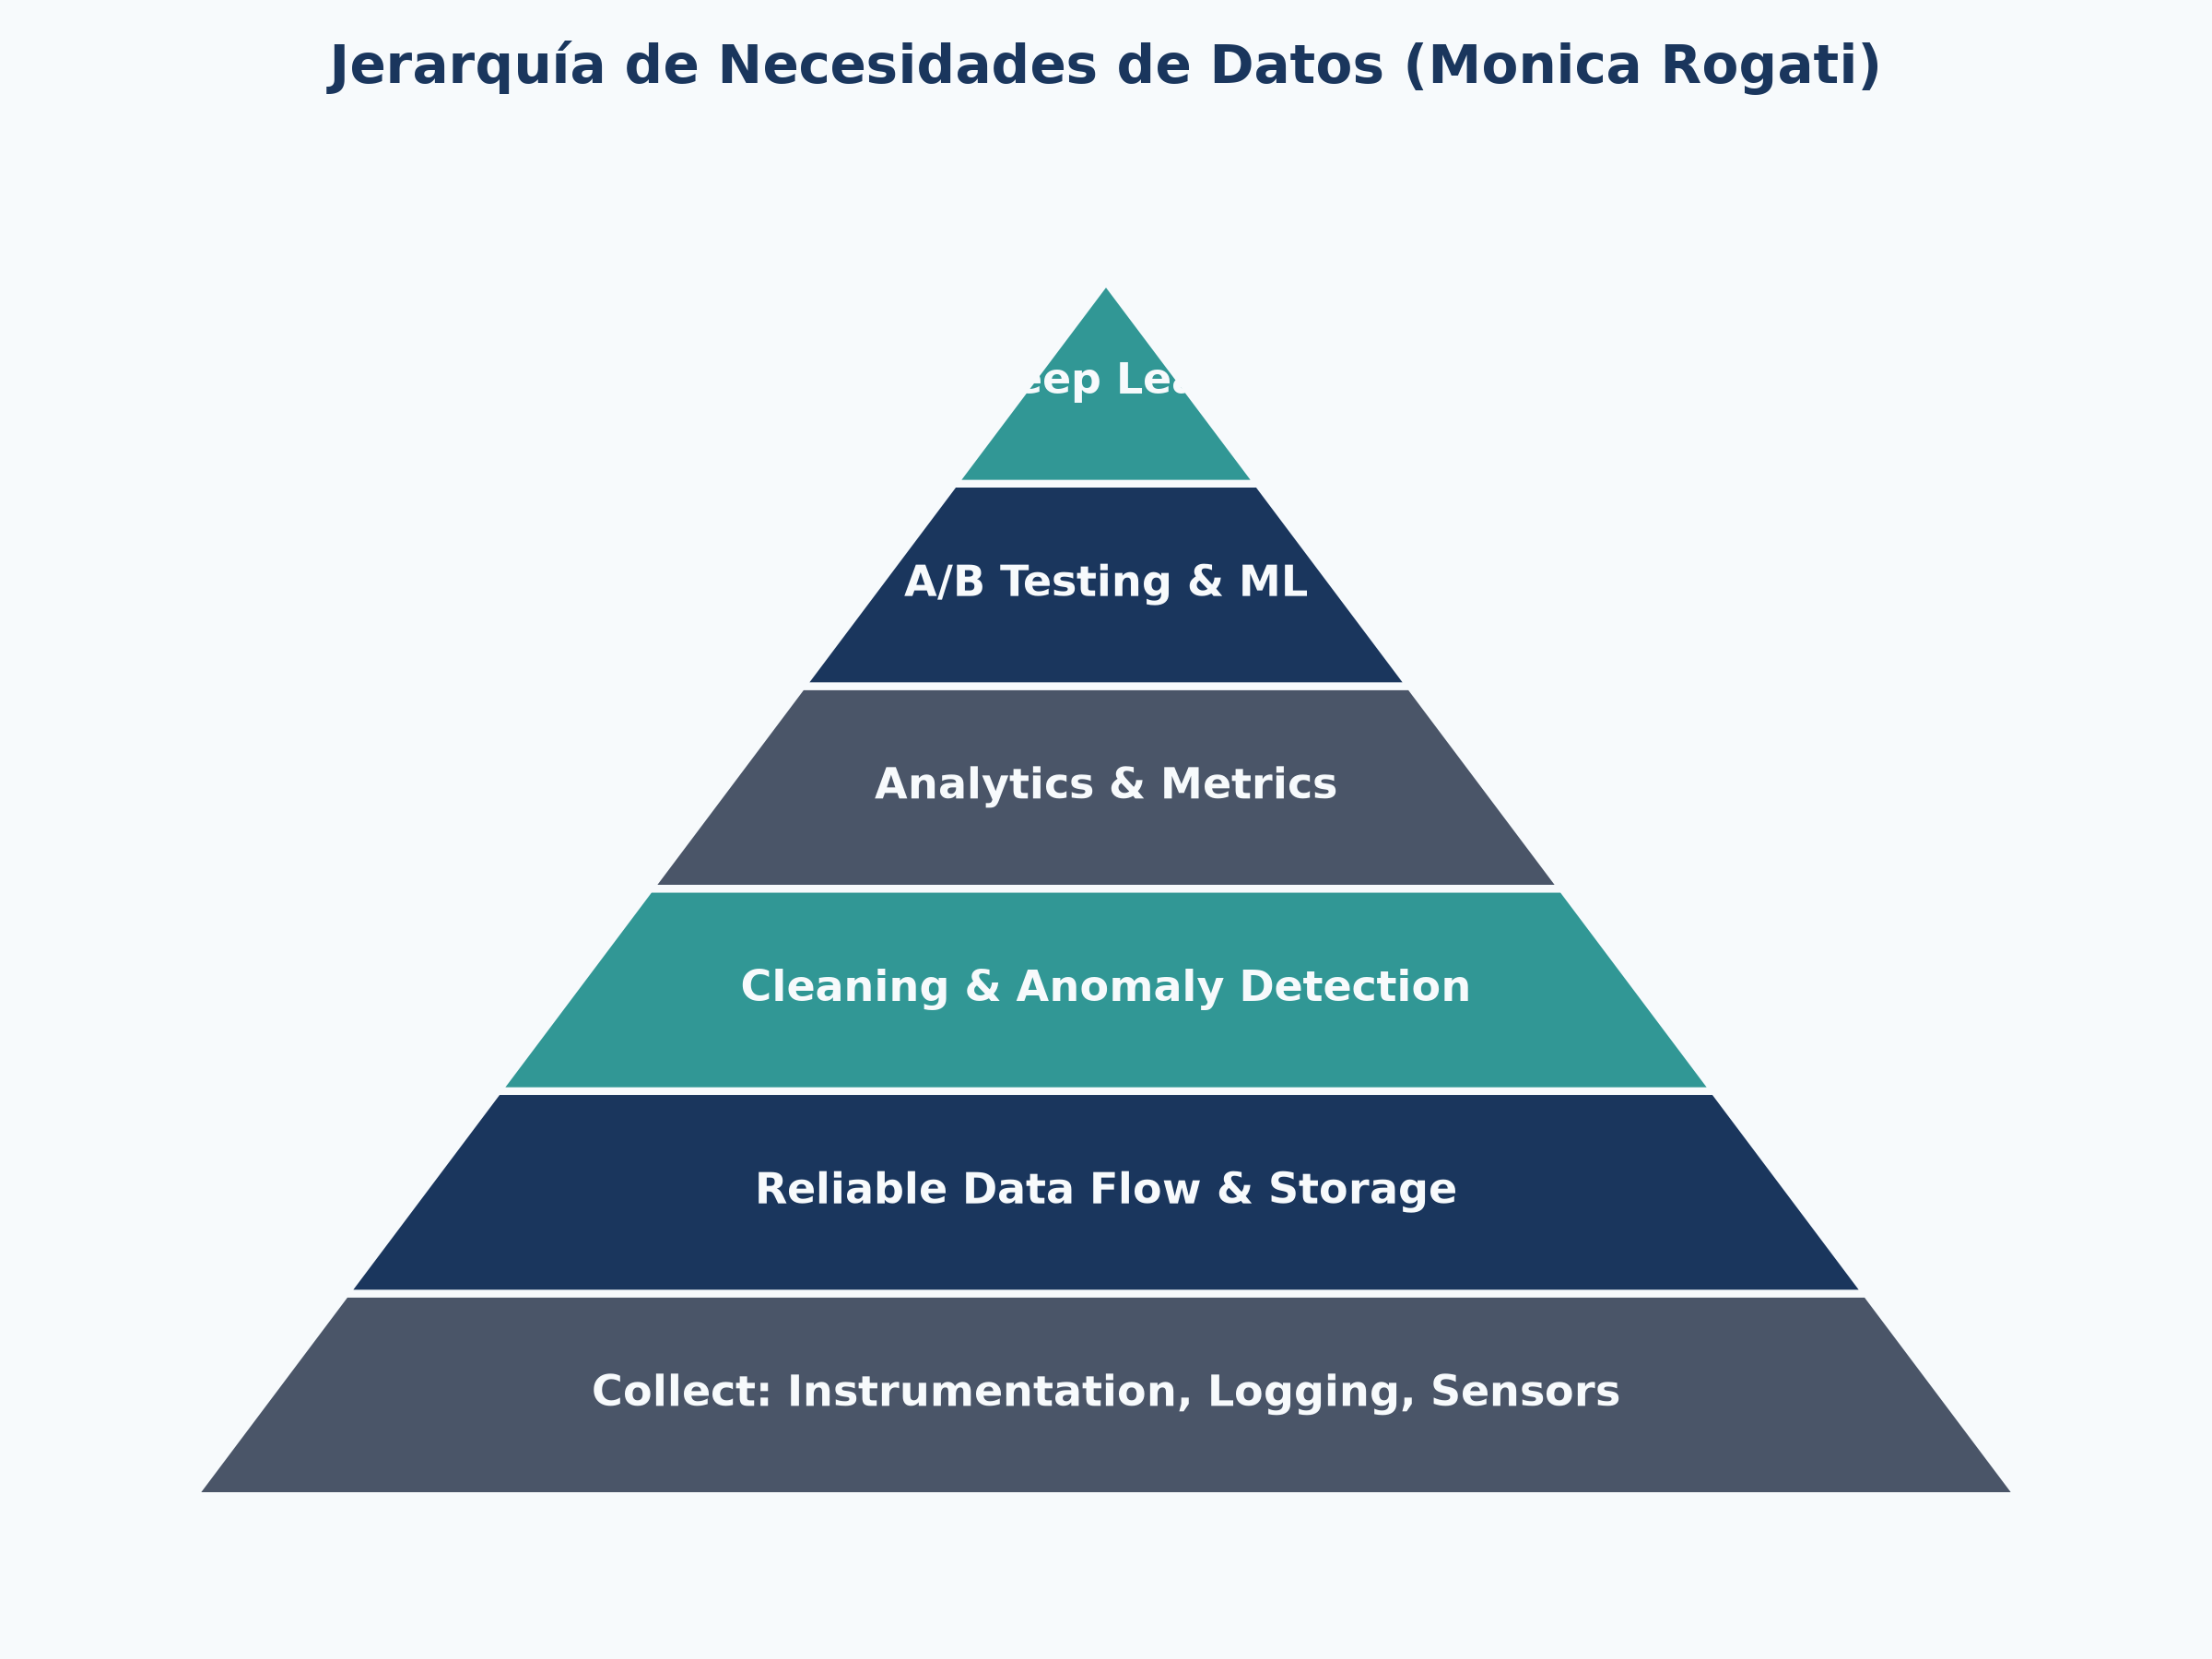
\includegraphics[width=0.55\textwidth]{jerarquia_datos.png}
    \end{center}
\end{frame}

\end{document}
